%************************************************
\chapter{Morfologia dei materiali polimerici}\label{ch:Morfologia}
%************************************************


%************************************************
\chapter{Proprietà meccaniche dei polimeri}\label{chp:MeccanicaPolimeri}
%************************************************
Tenendo conto del modello del gomitolo statistico a livello molecolare, vediamo come si classificano le proprietà meccaniche dei polimeri.
\begin{quote}
\emph{Come devono essere "costruiti" i polimeri in modo che si possano ottenere delle proprietà meccaniche interessanti?}
\end{quote}

Un primo modo può essere la strada degli additivi, del resto:\\
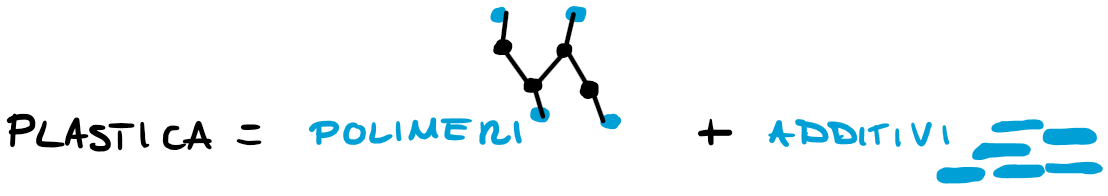
\includegraphics[width = \textwidth]{gfx/Plastica}\\
Un primo additivo usato per irrigidire un struttura polimerica è la fibra di vetro corta.
Vengono infuse nella plastica per migliorare le caratteristiche meccaniche.
Non se ne possono infondere troppe, altrimenti si perde il pregio della formabilità tipica dei materiali plastici.
Le \ac{FVC} vengono aggiunte fino al $40 \div 50\%$ in peso al polimero.

Esistono altre strade per poter migliorare le caratteristiche meccaniche dei polimeri;
\begin{description}
\item[Vincolo geometrico] Vincolare, in qualche modo, il materiale per evitare che il polimero formi la conformazione a gomitolo.
\item[Vincolo chimico] Si può pensare di irrigidire il polimero agendo sulle rotazioni relative delle molecole.
\item[Vincolo di legame] Agire sulla qualità dei legami intermolecolari.
\end{description}

\subsection{Vincolo geometrico}
Per evitare che le molecole ritornino alla forma di gomitolo statistico, si può formare delle fibre di materiale. Così viene limitato ad una certa geometria che, a meno di un piccolo ritorno elastico, non cambia la sua conformazione nel tempo.

Il motivo dell'aumento della resistenza è data dalla forma particolarmente allungata in cui le catene polimeriche vengono forzate.
Infatti, sebbene un minimo resta la conformazione a gomitolo, questo sarà particolarmente allungato. Tale conformazione permetterà alle forze applicate al polimero di agire di più sui legami di buona qualità piuttosto di quelli intermolecolari di qualità più scarsa.
Inoltre la fibra, essendo di piccolo spessore, prevede statisticamente meno difetti lungo la sezione. in pratica si limita la propagazione della frattura.

In particolare, questa pratica viene adottata per il \ac{PE}.

\subsection{Vincolo chimico}
Tenendo a mente la conformazione del \ac{PE}: se in catena principale vengono inseriti degli elementi che costituiscano dei legami covalenti a più alta energia in modo da limitare la rotazione relativa delle molecole.
Ad esempio si possono costituire legami doppi nella catena principale.
Il problema diventa l'instabilità dei legami doppi: tendono ad aprirsi molto facilmente.
Altra soluzione molto sfruttata sta nell'inserire anelli benzenici nella catena principale.
Stiamo parlando del \ac{PET}

\begin{figure}
\centering
\setchemfig{atom sep = 2em}
\chemfig{\vphantom{C}-[@{op,.75}]-C(=[6]O)-(**6(---(-C(=[6]O)-O-CH_2-CH_2-O-[@{cl,.25}])---))}
\polymerdelim[indice = n]{op}{cl}
\caption{Monomero del Polietilene tereftalato}
\label{fig:PET}
\end{figure}

La rigidezza del materiale è donato dall'anello benzenico. Infatti questo racchiude la maggior parte della massa del monomero. Inoltre è particolarmente rigido in quanto non sono permesse le rotazioni delle molecole componenti l'anello per via della risonanza.

Altro esempio di miglioramento del materiale grazie a vincoli chimici è quello del \ac{PPS}.
\begin{figure}
\centering
\setchemfig{atom sep = 2em}
\chemfig{\vphantom{C}-[@{op,.75}]**6(---(-S-[@{cl,.25}])---)}
\polymerdelim[indice = n]{op}{cl}
\caption{Monomero del Polifenilen solfuro}
\label{fig:PPS}
\end{figure}
Le caratteristiche così interessanti sono donate dal fatto che il monomero è praticamente un anello benzenico.
In entrambi i casi si parla di \textbf{Irrigidimento della catena principale}.

Non è l'unica soluzione: si possono aggiungere elementi rinforzanti come sostituenti laterali. In genere si usano elementi pesanti o ingombranti.
In questo caso viene limitato lo scorrimento relativo delle molecole per via dell'ingombro degli anelli benzenici, ad esempio.
Vengono limitate le rotazioni e gli scorrimenti relativi delle molecole per effetto degli ingombri dei sostituenti laterali

\begin{figure}
\centering
\setchemfig{atom sep = 2em}
\chemfig{\vphantom{C}-[@{op,.75}]CH_2-CH(-[6]**6(------))-[@{cl,.25}]}
\polymerdelim[indice = n]{op}{cl}
\caption{Irrigidimento dei sostituenti laterali}
\label{fig:IrrigidimentoLaterali}
\end{figure}

Ma:
\begin{itemize}
\item non si arriva al livello di irrigidimento che si ottiene tramite rinforzo in catena principale.
\item Il materiale ne risulta più fragile (per effetto dei vincoli dati dai sostituenti).
\end{itemize}
Questa tecnica viene detta di \textbf{irrigidimento dei sostituenti laterali}.

\subsection{Vincolo intermolecolare}
Le possibilità in questo caso sono due:
\begin{enumerate}
\item incrementare il numero di legami intermolecolari;
\item incrementare la qualità dei legami intermolecolari;
\end{enumerate}

\paragraph{Incremento numero dei legami}
Prendendo il caso del \ac{PE}: i legami intermolecolari sono di pessima qualità, principalmente \ac{FdW}. Aumentandone il numero risulta in una sommatoria "più lunga" di legami intermolecolari, permettendo un numero di vincoli maggiori.
Vengono realizzate delle catene principali estremamente lunghe.
In questo modo aumentano i "grovigli" che bloccano le catene rispettivamente.
Sempre nel \ac{PE}, si realizzano materiali ad alto grado di polimerizzazione $n \uparrow\uparrow$.
Però aumenta, contemporaneamente, il \ac{PM}:
\begin{equation}
P.M. = P_{\textup{monomero}} * n
\end{equation}

Aumentando il grado di polimerizzazione, le caratteristiche meccaniche aumentano, come si vede in figura \ref{fig:PMMeccanica}.
\begin{quote}
\emph{\dots Però\dots}
\end{quote}

Come si vede dalla figura \ref{fig:ViscPM}, contemporaneamente aumenta anche la viscosità del fluido.

\begin{figure}
\centering
\subfloat[][\emph{Andamento delle caratteristiche meccaniche in funzione del \ac{PM}}\label{fig:PMMeccanica}]
{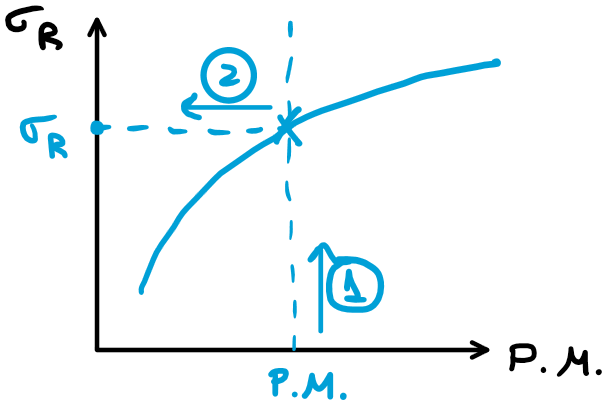
\includegraphics[width = 0.4\textwidth]{gfx/PMMeccanica}}\quad
\subfloat[][\emph{Andamento della viscosità in funzione del \ac{PM}}\label{fig:ViscPM}]
{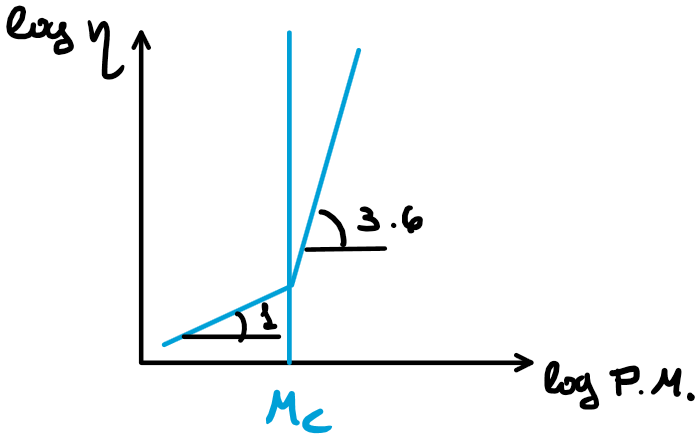
\includegraphics[width = 0.4\textwidth]{gfx/ViscPM}}
\caption{Confronto sull'aumento di \ac{PM} con le caratteristiche meccaniche e viscosità}
\label{fig:ConfPM}
\end{figure}

Nella pratica si fa una scelta in base alla viscosità che serve del polimero, da cui derivano determinate caratteristiche meccaniche.
Ciò è dovuto al fatto che le tecnologie con cui si lavorano i polimeri, necessitano di determinate viscosità per funzionare correttamente.
Ad esempio: nello stampaggio ad iniezione serve una viscosità bassa (per garantire il riempimento dello stampo) altrimenti il fluido non entra.
Mentre per l'estrusione serve una viscosità più alta.

Riassumendo, si sceglie la viscosità sulla base della lavorazione, da quella viscosità si ottengono determinate caratteristiche meccaniche.

\paragraph{Incremento qualità dei legami}
Il concetto è di sfruttare dei legami intermolecolari a più alta energia, ad esempio passando da \ac{FdW} a legami idrogeno. Oppure sfruttare una maggiore elettronegatività per rafforzare le \ac{FdW}.
Questo è il caso del \ac{PVC}: risulta un maggiore "attrito" tra le molecole data la presenza del cloro. Ciò è dovuta alla differente elettronegatività tra cloro e idrogeno, per cui ne risulta \ac{FdW} di miglior qualità.

Altro esempio di questo genere sono le \ac{PA}6 in confronto alle \ac{PA}12.
Nel \ac{PA}6 è più frequente il gruppo ammidico
{\setchemfig{atom sep = 2em}\chemfig{C(=[2]O)-N(-[2]H)}}
il quale è il responsabile della creazione del legame idrogeno.

\begin{figure}
\centering
\setchemfig{atom sep = 2em}
\chemfig{\vphantom{C}-[@{op,.75}]CH_2-CH_2-CH_2-CH_2-CH_2-C(=[2]O)-N(-[2]H)-[@{cl,.25}]}
\polymerdelim[indice = n]{op}{cl}
\caption{Poliammide 6}
\label{fig:PA6}
\end{figure}

%************************************************
\chapter{Classificazione dei polimeri}\label{chp:Classificazione}
%************************************************
Una prima classificazione dei materiali polimerici può essere fatta in base al loro comportamento di fluidificazione e/o indurimento:
\begin{description}
\item[Materiali termoplastici] sono tutti quei materiali che vengono scaldati per tornare allo stato fluido (anche se ad ogni ciclo si ha un degrado delle caratteristiche meccaniche)
\item[Materiali termoindurenti] sono materiali reticolati che necessitano di un processo di riscaldamento per poter ottenere il prodotto definitivo (ad esempio gli pneumatici). I legami dei reticoli sono di tipo covalente, infatti sono materiali dalle caratteristiche meccaniche interessanti.
\end{description}
Sebbene le caratteristiche meccaniche dei materiali termoindurenti siano di gran lunga superiori rispetto a quelli dei termoplastici, la loro produzione è più lenta per il fatto che la reticolazione chiede tempo.

Altra classificazione è basata sulla morfologia della catena principale:
\begin{description}
\item[Lineari] la catena principale non presenta ramificazioni o reticolazioni
\item[Ramificati] la catena principale si sviluppa su diverse linee. Bisogna considerare che la differenza tra sostituente laterale e ramificazione sta nella lunghezza dell'aggiunta laterale alla principale. Ad esempio un singolo anello benzenico non è una ramificazione ma solo un sostituente laterale.
\item[Reticolato] tutti i materiali termoindurenti presentano questa classificazione
\end{description}

Anche il metodo con cui si sintetizzano i polimeri ne classifica la specie:
\begin{description}
\item[Poliaddizione] detta anche polimerizzazione a catena
\item[Policondensazione] detta anche polimerizzazione a stadi
\end{description}

\paragraph{Poliaddizione}\label{par:Poliaddizione}
Tipicamente si apre un doppio legame della molecola da polimerizzare che legherà con molecole vicine, realizzando la catena principale.
È un processo tipico dei \textbf{vinili}.
Ad esempio la formaldeide crea delle catene di formaldeide aprendo il doppio legame tra metilene e l'ossigeno creando una catena di \ac{POM}. Il processo viene evidenziato in figura \ref{fig:Poliaddizione}.
Viene anche chiamata resina acetalica. 
Non più ampiamente utilizzata per via della tossicità della formaldeide.

\begin{figure}
\centering
\setchemfig{arrow coeff = 1.8, atom sep = 2em}
\schemestart
\chemfig{C(-[3]H)(-[5]H)=O} \arrow{->[poliaddizione]}
\chemfig{\vphantom{CH_2}-[@{op,.75}]C(-[2]H)(-[6]H)-O-[@{cl,.25}]}
\polymerdelim[height = 25pt, depth = 25pt, indice = n]{op}{cl}
\schemestop
\caption{Esempio di poliaddizione}
\label{fig:Poliaddizione}
\end{figure}

Ci sono delle variazioni sul processo di poliaddizione, ad esempio i \textbf{poliuretani} sono realizzati tramite l'incrocio delle due tecniche.

\paragraph{Policondensazione}\label{par:Policondensazione}
Speso non c'è una sola specie polimerica ma anche più.
Allora si creano dei polimeri, anche di specie diversa, in più si ottengono altri prodotti a basso peso molecolare dalla condensazione dei reagenti. Per esempio dalla condensazione del \ac{PET} si ottiene acqua. Vedi figura \ref{fig:Policondensazione}.

Il limite di tale processo è che le catene polimeriche non possono essere ad altissimo grado polimerico per via del fatto che del materiale viene impiegato come scarto.

\begin{figure}
\begin{minipage}{\textwidth}
\centering
\setchemfig{atom sep = 2em}
\schemestart
\chemname{\chemfig{C(=[3]C)(-[5]HO)-**6(---(-C(=[1]O)(-[7]OH))---)}}{Acido tereftalico}\+%
\chemname{\chemfig{HO-CH_2-CH_2-OH}}{Glicole etilenico} 
\arrow{->[Policondensazione]}[-90,2.5]
\chemname{\chemfig{\vphantom{C}-[@{op,.75}]O-C(=[2]O)-**6(---(-C(=[2]O)-O-CH_2-CH_2-[@{cl,.25}])---)}}{Poliestere tereftalato}
\polymerdelim[indice = n]{op}{cl} \+%
\chemname{\chemfig{H_2O}}{Acqua}
\schemestop
\end{minipage}
\caption{Policondensazione del \ac{PET}}
\label{fig:Policondensazione}
\end{figure}

Anche il \ac{PA}6 e \ac{PA}66 vengono realizzati tramite policondensazione.

Prendiamo ora in esame la realizzazione della catena polimerica più utilizzata oggigiorno:

\paragraph{Poliaddizione del PLA}
Il \ac{PLA} è una plastica utilizzatissima oggigiorno per via del fatto che è compostabile.
Attenzione: non è disperdibile in ambiente, necessita di determinate condizioni per poter essere elaborato in compost.

\begin{figure}
\centering
\setchemfig{atom sep = 2em}
\schemestart
\chemname{\chemfig{HO-C(-[2]CH_3)(-[6]H)-C(=[1]O)(-[7]OH)}}{acido lattico}%
\arrow{->[poliaddizione]}[0,1.5]%
\chemname{\chemfig{\vphantom{C}-[@{op,.75}]CH(-[2]CH_3)-C(=[2]O)-O-[@{cl,.75}]}}{\ac{PLA}}
\polymerdelim[indice +n]{op}{cl}
\schemestop
\caption{Poliaddizione del \ac{PLA}}
\label{fig:PoliaddizionePLA}
\end{figure}

Le molecole non sono uguali ma speculari (anche se non si vede dalla figura\ref{fig:PoliaddizionePLA}). C'è un problema di simmetria per via dell'ibridazione $sp3$ del carbonio.
Se durante la sintesi si mescolano diversi tipi di acidi polilattici ne esce un polimero poco regolare. Questo, si vedrà in seguito, determina la possibilità se il polimero potrà cristallizzare o meno.
In generale, un materiale polimerico può cristallizzare se, e soltanto se, è regolare.
Questa è una \textbf{condizione necessaria ma non sufficiente}.
Il PLLA e PDLA sono conformazioni del \ac{PLA} che possono cristallizzare perché regolari.
Il PLDLA no, questo è il \ac{PLA} irregolare, di più bassa qualità.

\section{Omopolimeri e copolimeri}
La condizione di omopolimeri e copolimeri dipende dalla conformazione della catena principale del polimero.
ipotizzando due monomeri $A$ e $B$ di una qualsiasi molecola, le possibili conformazioni sono quelli mostrati

\begin{figure}
\setchemfig{atom sep = 2em}
\schemestart
\chemname{\chemfig{\vphantom{A}-[@{op,.75}]A-A-A-A-A-A-[@{cl,.25}]}}{omopolimero}\polymerdelim[indice +n]{op}{cl}
\schemestop
\\\bigskip
\schemestart
\chemname{\chemfig{\vphantom{A}-[@{op,.75}]A-B-A-B-A-B-[@{cl,.25}]}}{copolimero alternato}\polymerdelim[indice +n]{op}{cl}
\schemestop
\\\bigskip
\schemestart
\chemname{\chemfig{\vphantom{A}-[@{op,.75}]A-A-A-B-B-B-[@{cl,.25}]}}{copolimero a blocchi}\polymerdelim[indice +n]{op}{cl}
\schemestop
\\\bigskip
\schemestart
\chemname{\chemfig{\vphantom{A}-[@{op,.75}]A-A-A-B(-[6]B(-[6]B-[6]))-[@{cl,.25}]}}{copolimero innestato}\polymerdelim[indice +n]{op}{cl}
\schemestop
\\\bigskip
\schemestart
\chemname{\chemfig{\vphantom{A}-[@{op,.75}]A-A-B-A-B-B-[@{cl,.25}]}}{copolimero random}
\polymerdelim[indice +n]{op}{cl}
\schemestop
\caption{Esempi di omopolimero e copolimero}
\label{fig:OmopolimeroCopolimero}
\end{figure}
